\begin{frame}[fragile]{Tutorial: Two-site fidelity optimization}

\begin{columns}

\begin{column}{5cm}

\begin{onlyenv}<1->
\begin{lstlisting}[language=JuliaLocal, style=julia, mathescape, basicstyle=\scriptsize\ttfamily]
$\psi$0 = Zp1*Zp2
$\psi$ = (Zp1*Zp2 + Zm1*Zm2)/√2



function F($\theta$)
  $\psi\theta$ = apply(U($\theta$,i1,i2),$\psi$0)
  return -abs2(inner($\psi$,$\psi\theta$))
end
$\partial$F($\theta$) = gradient(F, $\theta$)[1]
\end{lstlisting}
\end{onlyenv}

\begin{onlyenv}<3->
\begin{lstlisting}[language=JuliaLocal, style=julia, mathescape, basicstyle=\scriptsize\ttfamily]
$\theta$0 = [0, 0, 0, 0]
$\theta$ = minimize(F, $\partial$F, $\theta$0;
          nsteps=50, $\gamma$=0.1)

F($\theta$0) == -0.5
F($\theta$) # $\approx$ -0.9938992 $\approx$ -1
\end{lstlisting}
\end{onlyenv}

\end{column}

\begin{column}{5cm}

\begin{onlyenv}<1-1>
Reference state: \\
|0$\rangle$ = |Z+Z+$\rangle$ \\
~\\
Target state: \\
|$\psi\rangle$ = (|Z+Z+$\rangle$ + |Z-Z-$\rangle$)/√2 \\
~\\
$\min_{\theta}$ F($\theta$) = \\
\ \ \ \ \ \ $\min_{\theta}$ -|$\langle\psi$|U($\theta$)|0$\rangle$|$^2$
\end{onlyenv}

\begin{onlyenv}<2->
\vspace*{0.0cm}
\begin{center}
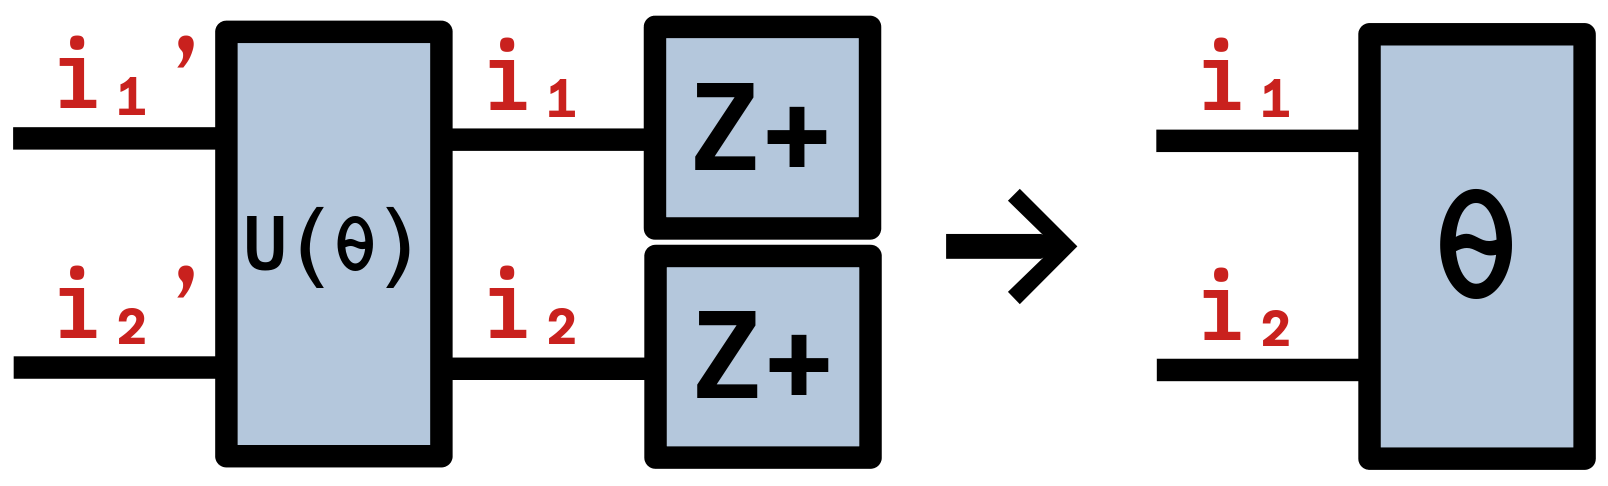
\includegraphics[width=1.0\textwidth]{
  slides/assets/UZp1Zp2.png
} \\
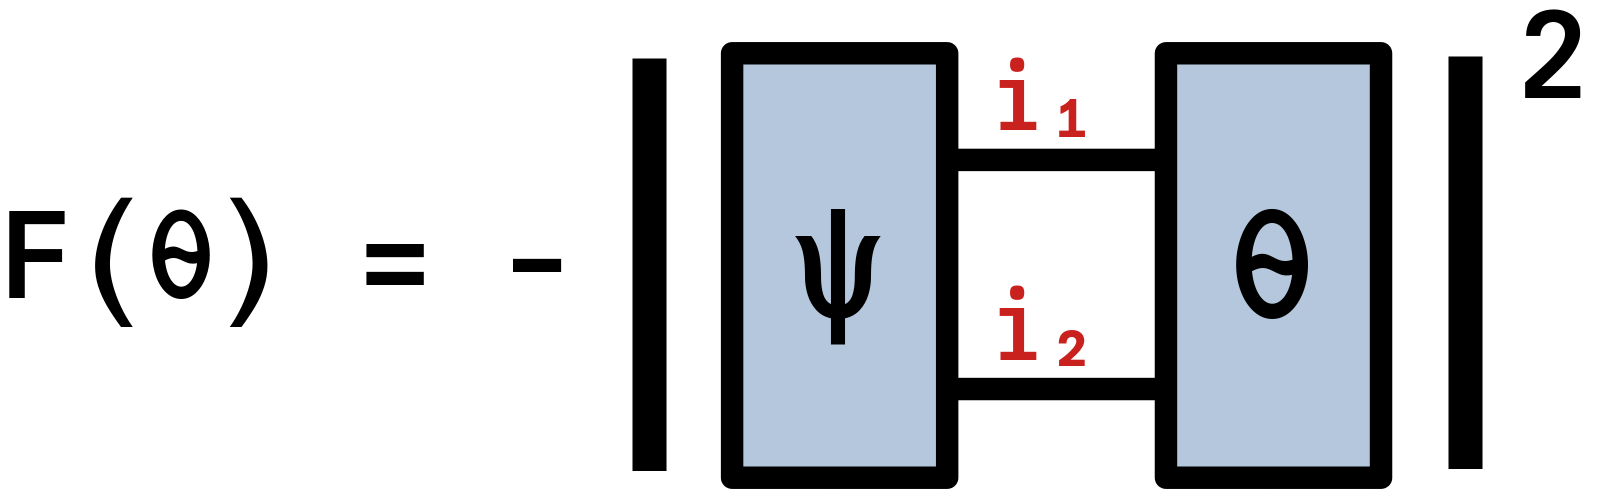
\includegraphics[width=1.0\textwidth]{
  slides/assets/psi12theta12.png
}
\end{center}
\vspace*{0.0cm}
\end{onlyenv}

\begin{onlyenv}<3->
\vspace*{0.0cm}
\begin{center}
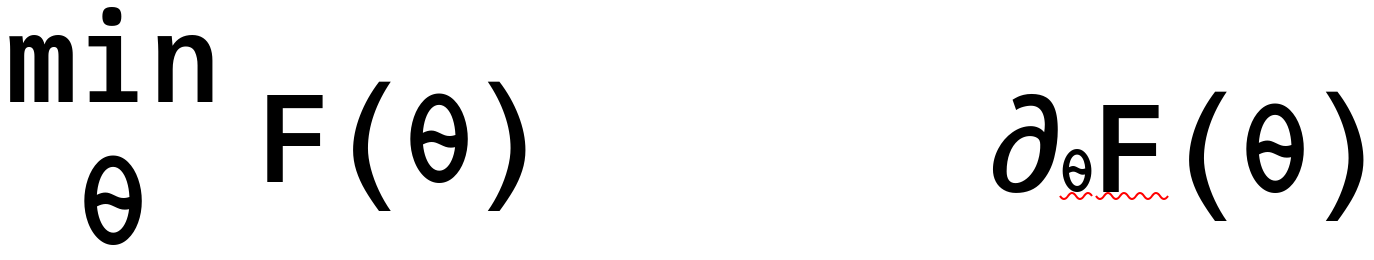
\includegraphics[width=1.0\textwidth]{
  slides/assets/min_grad_F_theta.png
}
\end{center}
\vspace*{0.0cm}
\end{onlyenv}

%% \begin{onlyenv}<4->
%% ~\\
%% ~\\
%% ~\\
%% ~\\
%% $\approx$ (-0.5, 0.5) \\
%% $\approx$ (-0.9938992, 0.07786879) \\
%%     $\approx$ (-1, 0)
%% \end{onlyenv}

\end{column}

\end{columns}

\end{frame}
